\documentclass{ximera}

\addPrintStyle{..}

\begin{document}
	\author{Bart Lambregs}
	\xmtitle{Vraagstukken}{}
    \xmsource\xmuitleg


\begin{exercise}
	Hoe groot is de snelheid die een slee met een massa van \SI{5,0}{kg} krijgt, als er gedurende \SI{6,0}{s} een kracht van \SI{0,20}{N} horizontaal op inwerkt?

	\begin{oplossing}
		\SI{0,24}{m/s}
	\end{oplossing}
\end{exercise}

\begin{exercise}
    Twee blokken met respectievelijke massa's $m_1$ en $m_2$ rusten op een horizontaal vlak. De wrijving tussen de blokken en het horizontale vlak mag verwaarloosd worden. Op \'e\'en van de blokken wordt een horizontale kracht $\vec{F}$ uitgeoefend zoals op de figuur is weergegeven. De kracht die blok 1 op blok 2 uitoefent is dan:

\begin{minipage}[t]{0.4\textwidth}
    \begin{multipleChoice}
        \choice{$\frac{m_1}{m_2}\vec{F}$}
        \choice{$\frac{m_1}{m_1+m_2}\vec{F}$}
        \choice[correct]{$\frac{m_2}{m_1+m_2}\vec{F}$}
        \choice{$\vec{F}$}
    \end{multipleChoice}
\end{minipage}
\hfill
\begin{minipage}[t]{.37\linewidth}
	\raisebox{1ex-\height}{%
		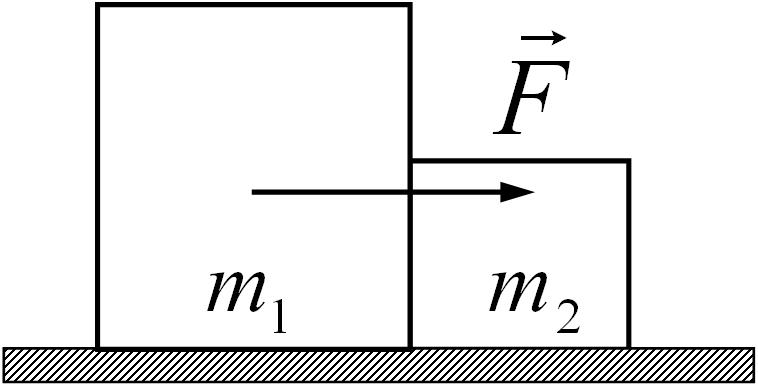
\includegraphics[width=\textwidth]{tweeblokken}} 
\end{minipage}
\end{exercise}

\begin{exercise}
    Een doos van \SI{10}{kg} wordt met een kracht van \SI{40}{N} over een glad tafeloppervlak getrokken. De uitgeoefende kracht maakt een hoek van $\SI{30}{\degree}$ met de horizontaal. Als de wrijving mag worden verwaarloosd, bepaal dan
   
    \begin{minipage}[t]{.6\linewidth}
        \begin{enumerate}
        \item de versnelling van de doos,
        \item de grootte van de normaalkracht, die de tafel op de doos uitoefent.
        \end{enumerate}
    \end{minipage}
    \begin{minipage}[t]{.4\linewidth}
        \vtop{%
            \vskip-1ex
                \hbox{%
                    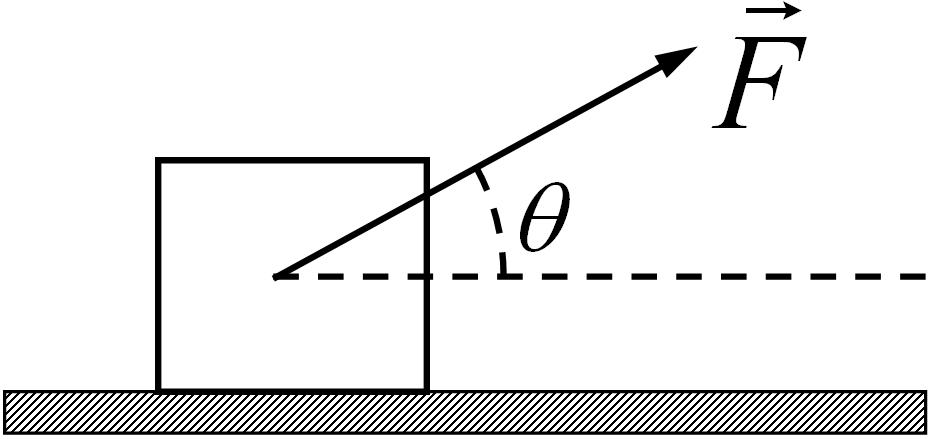
\includegraphics[width=\linewidth]{doos_kracht}%
            }%
        }
    \end{minipage}

    \begin{oplossing}
        \begin{enumerate}
            \item $a=\frac{F\cos\theta}{m}=\SI{3,46}{m/s^2}$
            \item $F_n=mg-F\sin\theta=\SI{78,1}{N}$
        \end{enumerate}
    \end{oplossing}
\end{exercise}

\begin{exercise}
    Een gewicht van \SI{225}{N} is bevestigd in het midden van een sterk touw. Door aan beide kanten een even grote kracht uit te oefenen wordt het gewicht opgetild. Bepaal de grootte van die krachten opdat het gewicht zoals in de figuur met $\theta=\SI{10}{\degree}$ komt te hangen.

    \begin{image}
        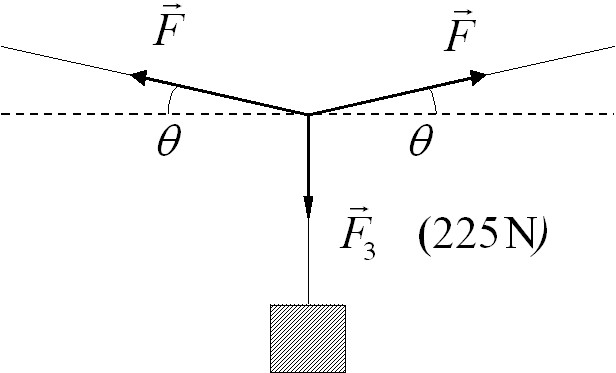
\includegraphics[width=\textwidth]{horizontaal_touw}
    \end{image}
\end{exercise}
	
\begin{exercise}{(\textbf{Toestel van Atwood})}
    Twee verschillende massa's zijn via een katrol van te verwaarlozen massa met elkaar verbonden zoals in de figuur. De wrijving is eveneens te verwaarlozen. 

    \begin{image}
        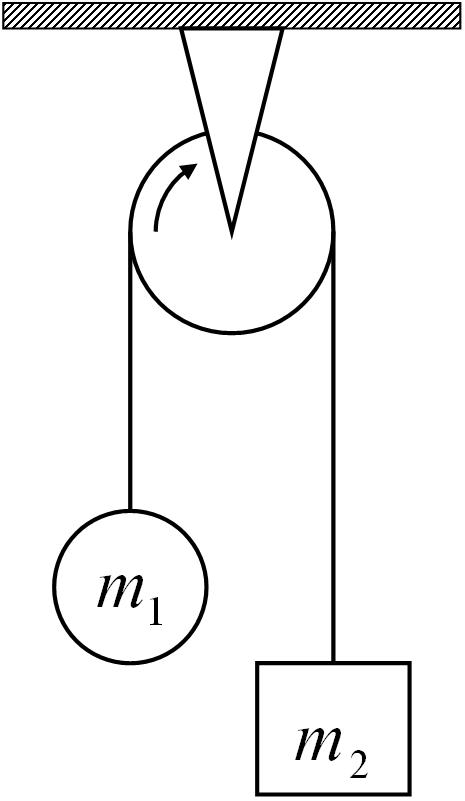
\includegraphics[height=2cm]{toestelatwood}
    \end{image}

    Bepaal de grootte van de versnelling van beide massa's en de spankracht in het touw.

    \begin{oplossing}
        $a=\frac{m_2-m_1}{m_1+m_2}g \quad F_s=\frac{2m_1m_2}{m_1+m_2}g$
    \end{oplossing}
\end{exercise}

\begin{exercise}
    Twee massa's $m_1$ en $m_2$ zijn via een touwtje en een katrol van te verwaarlozen massa met elkaar verbonden zoals in de figuur. Er is geen wrijving aanwezig. De massa's hebben een versnelling zoals aangegeven.

    \begin{image}
        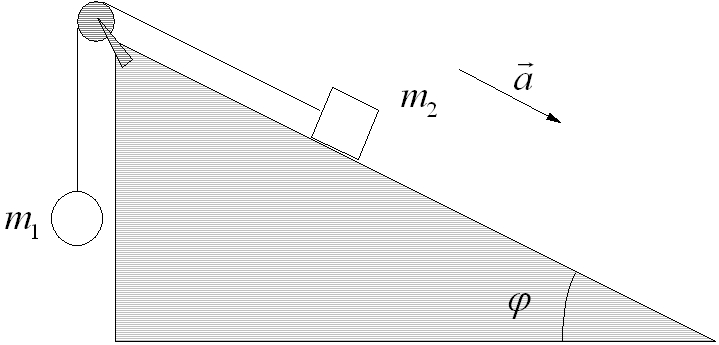
\includegraphics[width=.7\textwidth]{blokken_helling}
    \end{image}

    Bepaal de grootte van de versnelling van beide massa's en de grootte van de spankracht in het touw.
\end{exercise}

\begin{exercise}
	Hoe kan een man die \SI{686}{N} weegt langs een touw naar beneden glijden, dat slechts \SI{600}{N} kan dragen zonder te breken?

	Stel dat de man inschat dat hij, zonder zijn botten te breken, in staat is te springen van toch wel \SI{3,0}{m} hoog. Van hoe hoog zou hij dan met een dergelijk touw kunnen ontsnappen?

	\begin{oplossing}
		Door niet met zijn volle gewicht aan het touw te gaan hangen kan de man verhinderen dat het touw breekt. Het gevolg is wel dat hij een nettokracht naar beneden ondervindt waardoor hij toch naar beneden versnelt, al is het met een kleinere versnelling dan de valversnelling.

		Door met \SI{600}{N} aan het touw te trekken, ondervindt hij een spankracht omhoog met diezelfde grootte. Met een referentieas naar beneden volgt uit $F_z-F_s=ma$ en uit $m=\frac{F_z}{g}$ voor de versnelling van de man:
		\begin{equation}
			a=\left(1-\frac{F_s}{F_z}\right)g\label{versnelling_ontsnapper}
		\end{equation}
		wat gelijk is aan \SI{1,23}{m/s^2}.

		Uit $v^2=v_0^2+2ax$ volgt de maximale snelheid die hij bij de impact op de grond aankan als we voor $a$ de valversnelling $g$ nemen en voor $x$ de gegeven \SI{3,0}{m}. Uit diezelfde formule vinden we de hoogte $h$ vanwaar de man kan ontsnappen als we nu de netto versnelling $a=\SI{1,23}{m/s^2}$ (\ref{versnelling_ontsnapper}) nemen: 
		\begin{equation*}
			h=\frac{v^2}{2a}=\ldots=\frac{F_z}{F_z-F_s}x
		\end{equation*}
		wat gelijk is aan \SI{24}{m}.
	\end{oplossing}
\end{exercise}

\begin{exercise}
    Een jager (massa \SI{70}{kg}) heeft een ijsbeer (massa \SI{350}{kg}) geschoten met een harpoen en wil die nu naar zich toe trekken met het touw. Jager en ijsbeer zijn oorspronkelijk allebei in rust op het ijsoppervlak en op \SI{30}{m} van elkaar. Verwaarloos de wrijving met het ijs. Bepaal de afstand waarover de ijsbeer is verschoven als de jager de ijsbeer binnenhaalt.
\end{exercise}
% Bron fysica olympiade ...?

\end{document}